\documentclass[aspectratio=169]{beamer}
\usetheme{hogent}
\usecolortheme{hgwhite} % witte achtergrond, zwarte tekst

%% common.tex -- Code die in elk .tex-bestand terug komt

%% Packages

\usepackage[dutch]{babel}
\usepackage{graphicx}
\usepackage{comment,enumerate,hyperref}
\usepackage{amsmath,amsfonts,amssymb}
\usepackage{eurosym}
\usepackage{booktabs}
\usepackage{multicol,multirow}
\usepackage{listings}

\usepackage[outputdir=out]{minted}
%\usepackage{minted}

\usepackage[backend=biber,style=apa]{biblatex}
\DeclareLanguageMapping{dutch}{dutch-apa}

\usepackage{csquotes}

%% Variabelen, elk academiejaar aan te passen
\newcommand{\academicyear}{2023--2024 (revisie: \today)}
\newcommand{\lecturers}{Thomas Aelbrecht \and Thomas Parmentier \and Bert Van Vreckem}
\newcommand{\coursename}{Research Methods (IT)}

%% Macro's en commando's

%% \alertbox: een kader voor tekst die moet opvallen
\newcommand{\alertbox}[2][hgblue]{%
  \setbeamercolor{alertbox}{bg=#1,fg=white}
  \begin{beamercolorbox}[sep=2pt,center]{alertbox}
    \textbf{#2}
  \end{beamercolorbox}
}

\addbibresource{rm4-bibliografie.bib}

%---------- Info over de presentatie ------------------------------------------

\title{Module 4. Creating a bibliographic database.}
\subtitle{\coursename}
\author{\lecturers}   % Pas waarden aan in common.tex
\date{\academicyear}

\begin{document}

\begin{frame}
  \maketitle
\end{frame}

\begin{frame}
  \frametitle{Content}

  \tableofcontents
\end{frame}

\section{Source citations and reference list in {\LaTeX} .}

\begin{frame}[plain]
	\frametitle{Reference list.}
	
	
	\begin{columns}[c]
		
		\column{.5\textwidth}
		Goal of a reference list is to allow readers to:
		
		
		\begin{itemize}
			\item Look up the cited sources
			\item Judge their quality
		\end{itemize}
		
		{\pause}
		
		Strict, fixed format:
		
		\begin{itemize}
			\item Formatting rules (eg. APA, Chicago Manual of Style, IEEE \ldots)
			\item Fixed order (by appearance or alphabetically)
			\item List of URLs does not suffice!
		\end{itemize}
		
		{\pause}
		
		\column{.5\textwidth}
		\begin{center}
			
\includegraphics[width=\columnwidth]{4/bibliography.png}
		\end{center}
		
	\end{columns}
	
	
	{\pause}
	
	\alertbox{Use \textcolor{hgyellow}{reference management software} to generate your reference list!}
	
\end{frame}

\begin{frame}
  \frametitle{Bibliografic database}

$\rightarrow$ Software to store sources in a structured manner
  \begin{itemize}
    \item Full text + metadata
    \item Generate correctly styled literature list
    \item Reference management software
  \end{itemize}
\end{frame}

\begin{frame}
  \frametitle{Examples}

  \begin{itemize}
    \item Endnote: commercial
    \item Mendeley: commercial, free
    \item JabRef: open source
  \end{itemize}

\end{frame}

\begin{frame}[plain]
  \frametitle{JabRef}

  \centering
  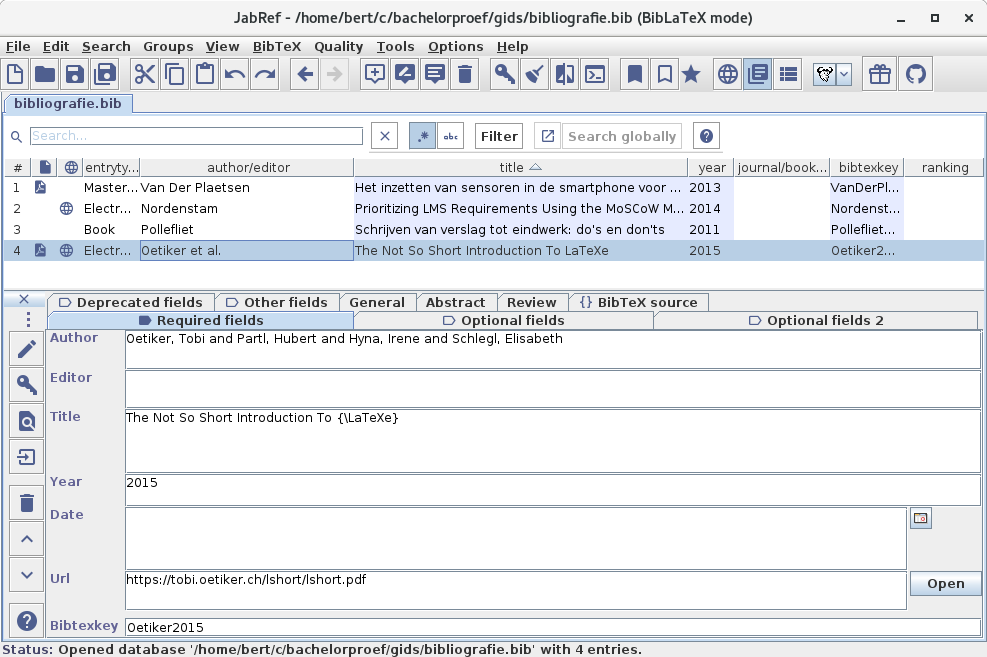
\includegraphics[height=.8\textheight]{4/jabref-screenshot}

\end{frame}

\begin{frame}
    \frametitle{JabRef settings}
    
   Options > Preferences

   \begin{itemize}
        \item General
        \begin{itemize}
            \item Default library mode: \textbf{biblatex}
        \end{itemize}
        \item Linked Files \textit{(optional)}
        \begin{itemize}
            \item Main file directory: (path to folder where you keep the PDF files)
        \end{itemize}
        \item{Entry Preview}
        \begin{itemize}
            \item Entry Preview: American Psychological Association 7th edition
        \end{itemize}
    \end{itemize}
    \bigskip
    In Dutch: \url{https://hogenttin.github.io/latex-hogent-gids/installatie-jabref/}
    
\end{frame}
\begin{frame}[fragile]
  \frametitle{Source citation and reference list in {\LaTeX}.}

  Bib{\LaTeX} and Biber

  \vspace{18pt}

  \verb|article.tex|: Main text\\
  \verb|article.bib|: Bibliografic database (edit using e.g.~JabRef)

  \bigskip

  Preamble:

  \begin{verbatim}
  \usepackage[backend=biber,style=apa]{biblatex}
  \DeclareLanguageMapping{english}{english-apa}
  \addbibresource{article.bib}
  \end{verbatim}

    \textbf{Remark:}\ Already in template!   

\end{frame}

\section{Creating a bibliographic database.}

\begin{frame}
  \frametitle{Bibliografic data in Jabref.}

  Fields that \textbf{always} need to be filled:

  \begin{description}
    \item[Author] Surname, Firstname and Surname, Firstname and Surname, Firstname \ldots
    \item[Title] of the article, book, \ldots
    \item[Year] or publication date
    \item[Bibtexkey] id of this source, used when referencing, (tip: click on the key icon)
  \end{description}
  \bigskip
  Impossible to fill in one of these fields? Then the source is probably unsuitable!
\end{frame}

\begin{frame}
  \frametitle{The author field}

  Always use this format:

  \begin{itemize}
    \item People: ``Surname, Firstname and Surname, Firstname and Surname, Firstname\ldots''
    \item Organisation: between curly brackets e.g.\ ``\{The Linux Foundation\}''
  \end{itemize}

\end{frame}

\begin{frame}[fragile]
  \frametitle{Bibliografic data in Jabref.}
  \framesubtitle{Extra fields for Article}

  \begin{description}
    \item[Journal] Name of the journal
    \item[Volume] Volume
    \item[Number] Number within the volume (optional)
    \item[Pages] \verb|mmm--nnn|
  \end{description}

  \bigskip

  \textbf{Example:}

  \fullcitebib{Anscombe1973}
\end{frame}

\begin{frame}
  \frametitle{Tip: fill in fields automatically}

  \begin{itemize}
    \item Elsevier, Springer, \ldots\ have Bib\LaTeX{} export function
    \item Paste in tab page ``BibTeX source''
  \end{itemize}

  \bigskip

  \centering
  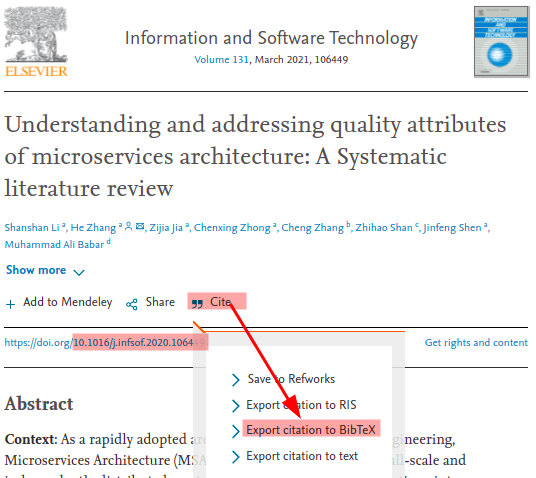
\includegraphics[height=.6\textheight]{4/elsevier-cite-doi}

\end{frame}

\begin{frame}
  \frametitle{Tip: fill in fields automatically}

  \begin{itemize}
    \item DOI = Digital Object Identifier
    \item Unique code for a publication
    \item Jabref: General > DOI > Get Bibtex data from DOI
  \end{itemize}

  \bigskip

  \centering
  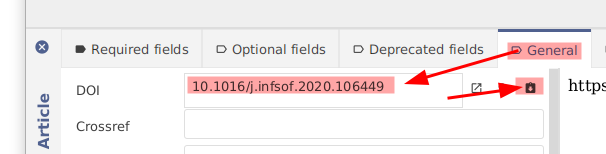
\includegraphics[height=.3\textheight]{4/jabref-doi}

\end{frame}

\begin{frame}[plain]
  \frametitle{Tip: fill in fields automatically}

  \centering
  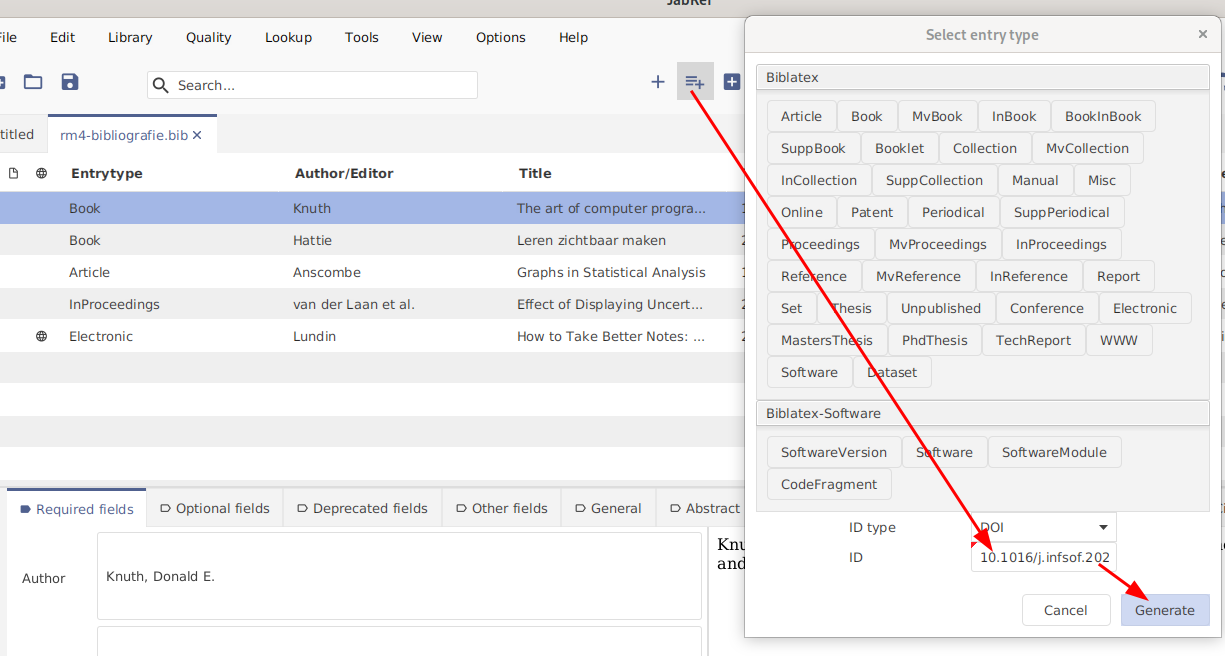
\includegraphics[height=.8\textheight]{4/jabref-new-entry-doi}

\end{frame}

\begin{frame}[plain]
  \frametitle{Bibliografic data in Jabref.}
  \framesubtitle{Extra fields for Electronic (Online, WWW)}

  \begin{description}
    \item[Url] Hyperlink to source
    \item[Urldate] Visit date
  \end{description}

  \bigskip

  \textbf{Example:}

  \bigskip

  \fullcitebib{Lundin2020}

\end{frame}

\begin{frame}[plain]
  \frametitle{Bibliografic data in Jabref.}
  \framesubtitle{Extra fields for InProceedings}

  \begin{description}
    \item[Booktitle] ``Proceedings of the [name conference]''
    \item[Editor] Editor(s) (optional)
    \item[Pages] Page numbers (optional)
  \end{description}

  \medskip

  \textbf{Example:}

  \fullcitebib{vanderLaanEtAl2015}
\end{frame}

\begin{frame}[plain]
	\frametitle{Bibliografic data in Jabref.}
	\framesubtitle{Extra fields for Book}
	
	\begin{description}
		\item[Publisher] Name of the publishing company
		\item[Address] of the publisher
	\end{description}
	
	\medskip
	
	Adding an URL is not customary for books, unless published online.
	
	Web page of the publisher is OK, Google Books or illegal mirrors are not.
	
	\medskip
	
	\textbf{Example:}
	
	\fullcitebib{Knuth1998}
\end{frame}

\begin{frame}
	\frametitle{Bibliografic data in Jabref.}
\framesubtitle{Extra fields for Report/Thesis}
	
	\begin{description}
		\item[Institution] or organisation
		\item[Type] Report type (dropdown in JabRef)
		\item[URL]  and Urldate (if published online)
	\end{description}
	
\end{frame}

\begin{frame}[plain]
	
	\textbf{Bachelor thesis example:}
	
	\fullcitebib{VanDerPlaetsen2013}
	
	\medskip
	
	\textbf{Research report example:}
	
	\fullcitebib{DeMarez2022}
	
\end{frame}

\begin{frame}
  \frametitle{Bibliografic data in Jabref.}

  Fill out as much information as possible (facilitates searching):

  \begin{description}
    \item[DOI] Digital Object Identifier: unique ID for article, automatically fill in every field
    \item[URL] even if it is not a real Electronic source
    \item[Keywords] Keywords
    \item[File] PDF of the publication
    \item[Abstract] Summary
    \item[Comments] Your own summary/remarks
  \end{description}

\end{frame}

\begin{frame}[fragile]
	\frametitle{URL cleanup}
	
	\begin{itemize}
		\item Trim optional URL parameters  
		\begin{itemize}
			\item Referral/tracking info
			\item Highlighting (\verb+https://URL#:~:text=HIGHLIGHT+)
		\end{itemize}
		\item Refer to the \textit{original} source
		\begin{itemize}
			\item Do \emph{NOT} use tertiairy sources (Google Books, Arxiv.org, CiteseerX \ldots)
		\end{itemize}
	\end{itemize}
	
\end{frame}

\section{Referencing literature.}

\begin{frame}[fragile]
  \frametitle{Referencing in the text}
  
  \begin{itemize}
  	\item When? $\rightarrow$ the first time you use the source
  	\item Where? $\rightarrow$ \textcolor{hgorange}{\textbf{within}} this first sentence
  \end{itemize}
  \bigskip
  Two different citations methods:

  \begin{itemize}
    \item \verb|\textcite{Knuth1998}| \(\Rightarrow\) Knuth (1998)
    \item \verb|\autocite{Knuth1998}| \(\Rightarrow\) (Knuth, 1998)
  \end{itemize}
\end{frame}

\begin{frame}[fragile,plain]
	\frametitle{Narrative reference}
	\framesubtitle{Use \texttt{\textbackslash{}textcite}}

  \ldots\ if the name of the author is part of the sentence:
  
\bigskip

\small
\begin{verbatim}
An overview is provided in the survey by~\textcite{RibasEtAl2010}.
For a real-life case-study of applying genetic algorithm ``on top''
of a Mixed Integer Linear Programming model, we refer
to~\textcite{BorodinEtAl2011}.
\end{verbatim}
\normalsize

\begin{center}
	$\Downarrow$
\end{center}

  \begin{quotation}
    An overview is provided in the survey by Ribas et al (2010). For a real-life case-study of applying genetic algorithm ``on top'' of a Mixed Integer Linear Programming model, we refer to Borodin et al (2011).
  \end{quotation}

\end{frame}

\begin{frame}[fragile]
	\frametitle{Reference between brackets}
	\framesubtitle{Use \texttt{\textbackslash{}autocite}}
	
	\ldots\ if the name of the author is NOT part of the sentence:
	
	\medskip
	
	\small
	\begin{verbatim}
Reinforcement Learning (RL) is a technique that allows an agent
to learn how to maximize a numerical reward
signal~\autocite{SuttonBarto1998}.
\end{verbatim}
	\normalsize
	
	\begin{center}
		$\Downarrow$
	\end{center}
	
	\begin{quotation}
		Reinforcement Learning (RL) is a technique that allows an agent to learn how to maximize a numerical reward signal (Sutton and Barto, 1998).
	\end{quotation}
	
	\bigskip
	
	Also for exact citations and image sources.
	
\end{frame}

\begin{frame}[fragile]
  \frametitle{Insert reference list.}

  \begin{itemize}
    \item Insert reference list: \verb|\printbibliography|

    \item Compile (in TexStudio):

          \begin{enumerate}
            \item Build/Compile (F5): sources are not added yet, ``keys'' of sources are marked in bold
            \item Bibliography (F8): selects the referenced sources and prepares them
            \item Build/Compile (F5): inserts references in the text and generates the reference list
          \end{enumerate}
	\item  In VSCode: use recipe \texttt{XeLaTeX $\rightarrow$ biber $\rightarrow$ XeLaTeX $\times$ 2}
  \end{itemize}
\end{frame}

\begin{frame}
  \frametitle{Check the result!}
  \begin{itemize}
  	\item Missing bibliography entries?
  	\begin{itemize}
  		\item Only cited sources get added
  		\item So use \texttt{{\textbackslash}textcite\{\}} or \texttt{{\textbackslash}autocite\{\}}
  		\item \texttt{Do \emph{not} use \texttt{{\textbackslash}nocite\{*\}}}
  	\end{itemize}
    \item Authors displayed correctly?
    \item No language errors or typos? E.g.\ accents or special characters
    \item All info needed to find source is present?
    \item Mentioning of ``Visited DATE, of URL'' for \textit{Online} sources?
    \item \textbf{Attention!} Special characters (\%,\$,\& \ldots) are prohibited in .bib files. Double-check this when importing sources with an abstract.
    \item \ldots
  \end{itemize}
\end{frame}

\begin{frame}[fragile]
	\frametitle{Tip: bibla}
	
	\begin{itemize}
		\item \url{https://pypi.org/project/bibla/}
		\item Linter/style checker for BibLaTeX files
		\item Checks for common errors
		\item By HOGENT alumnus Tristan Cuvelier
	\end{itemize}
	\bigskip
	\begin{verbatim}
     pip install bibla
     bibla lint bibliografie.bib
\end{verbatim}
	
\end{frame}

\begin{frame}
  \frametitle{Common mistakes}
  \framesubtitle{Reference list}

  \begin{itemize}
    \item Non-scientific sources used (e.g.\ StackOverflow, Wikipedia, blog not of a subject expert \ldots)
    \item Untrimmed URLs
    \item Incorrect or missing information (e.g. missing page numbers, wrong order of authors, wrong author \ldots)
    \item Incorrect citation type (e.g. \texttt{Online} instead of \texttt{Book} for a book)
    \item COPY \& PASTE OF TITLES IN ALL CAPS.
    \item URLs of illegal download sites
    \item Nonexistent sources generated by LLMs
    \item \ldots
  \end{itemize}
\end{frame}

\begin{frame}
 	\frametitle{Common mistakes}
	\framesubtitle{Citations}

\begin{itemize}
	\item Image without citation (= \textcolor{hgorange}{\textbf{Plagiarism!}})
	\item Statements or definitions without citation
	\item Citing sources which do not support the statement in the text
	\item Citing sources outside the (relevant) phrase.
	\item A single citation at the end of a paragraph
	\item Too much text based on a single source (max. a couple of sentences)
	\item \ldots
\end{itemize}
\end{frame}

\begin{frame}
	\frametitle{Common mistakes}
	\framesubtitle{Find the issues}
	
	\centering
	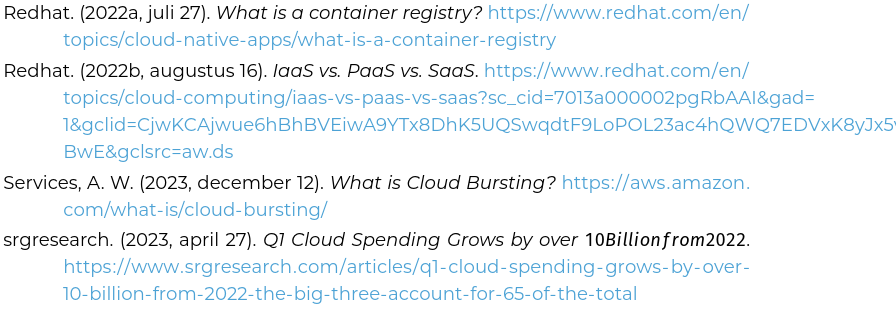
\includegraphics[height=.6\textheight]{4/jabref-dont.png}
	
	
\end{frame}

\begin{frame}[plain]
  \frametitle{Exercise}

  Save these sources in JabRef, with all necessary info and full text (where possible) and/or URL of the online source:

  \bigskip

  \begin{itemize}
    \item \url{https://www.sciencedirect.com/science/article/abs/pii/S0020025510002756}
    \item \url{https://catalogus.hogent.be/catalog/hog01:000617334}
    \item \url{https://martinfowler.com/articles/microservices.html}
    \item \url{https://www.youtube.com/watch?v=wW9CAH9nSLs&t=13s}
    \item \url{https://link.springer.com/book/10.1007/978-1-4842-6399-0}
    \item \url{https://link.springer.com/chapter/10.1007/978-3-031-27199-1_1}
    \item \url{https://docs.ansible.com/ansible-core/devel/index.html}
  \end{itemize}

\end{frame}

\begin{frame}
  \frametitle{Assignment}

  \begin{itemize}
    \item Save all found sources in .bib-file
    \item Structure, e.g.\ using Mind Map
          \begin{itemize}
            \item Freemind, Gitmind, Xmind, Minder, Vym, \ldots
          \end{itemize}
    \item Process what you read to a continuous text
  \end{itemize}

  \bigskip

  \alertbox{This is the most important phase of the assignment!}
\end{frame}

\end{document}
